\chapter{Introduction}\label{ch:introduction}
\epigraph{
- Homer, is it the way you pictured PhD life?\\
- Yeah, pretty much, except we drove in a van solving mysteries.
}{Could be Homer Simpson}

\begin{addmargin}[5em]{5em}
This thesis is situated in the research fields of data mining, constraint learning
and logic programming. We introduce each of them in turn and provide an overview of the
contributions of the thesis and
its general structure.
\end{addmargin}

\section{Data mining}\label{sec:data_mining}
The ability to write down a mathematical model and to simply push a button to get the
answer is an appealing idea. It is one of the holy grails of
Artificial Intelligence, called Declarative Programming, where one
specifies what the problem is and not how to solve it. Today in the age of data, we would like
to state what type of knowledge we are looking for, feed the data in and, as a result,
(almost magically) find new insights into the data. What we do not want is to write
a lot of tedious code. Unsurprisingly, this is a hard challenge. 


The \textit{knowledge} extracted from the data can manifest itself in
multiple forms. For example, an interesting piece of data,
\textit{typically a substructure}, is referred to as a \textit{pattern} \parencite{han_book}. 
The most known pattern learning task is 
\textit{frequent pattern mining}, or pattern mining for short
\parencite{survey_han}.
At a higher and more general level, often referred to as \textit{theory
mining}, it can be formalized as follows: \\

\newtheorem*{definition*}{Definition}

\begin{definition*}[Theory Mining]
\begin{mdframed}
Let $D$ be a dataset, $P$ be the language of allowed patterns and
$\phi$ be a predicate of
interest, the mining problem is then the problem of finding
all patterns $p$ in $P$ such that $\phi(p,D)$ holds.
\end{mdframed}
    %\label{def:mining}
\end{definition*}

Simply speaking, we enumerate objects that have a certain property of
interest. Various measures of relevance or ``interestingness'' of a pattern exist \parencite{tias_topk}.

The rest of the chapter is structured as follows. In Section
\ref{sec:data} we introduce two types of data used in data mining.
Then, in Section \ref{sec:rel_problems} we present types of relational pattern
mining problems that we investigate in this thesis. In Section
\ref{sec:declarative_intro}, we propose an approach to these problems,
while in Sections \ref{sec:logic_programming} and \ref{sec:cp_intro},
we present techniques for this approach to work. In Section
\ref{sec:common}, we demonstrate similarities and common traits of the
problems we investigate. We conclude with contributions in Section
\ref{sec:contributions} and links to experimental data and code in
Section \ref{sec:datasets}


\section{Propositional and relational data}\label{sec:data}
There are two common types of data in data mining: propositional and
relational. Propositional data is a in, so called, single-tuple
single-table format, where each row is an independent record and each
column is an attribute. It is commonly used in machine learning and data mining for training
models. Relational data, on the other hand, consists of  multiple
tables and there are constraints and dependencies between tables. This format is typically
more complex.

\pubrev
\begin{figure}[thb]
  \begin{center}
    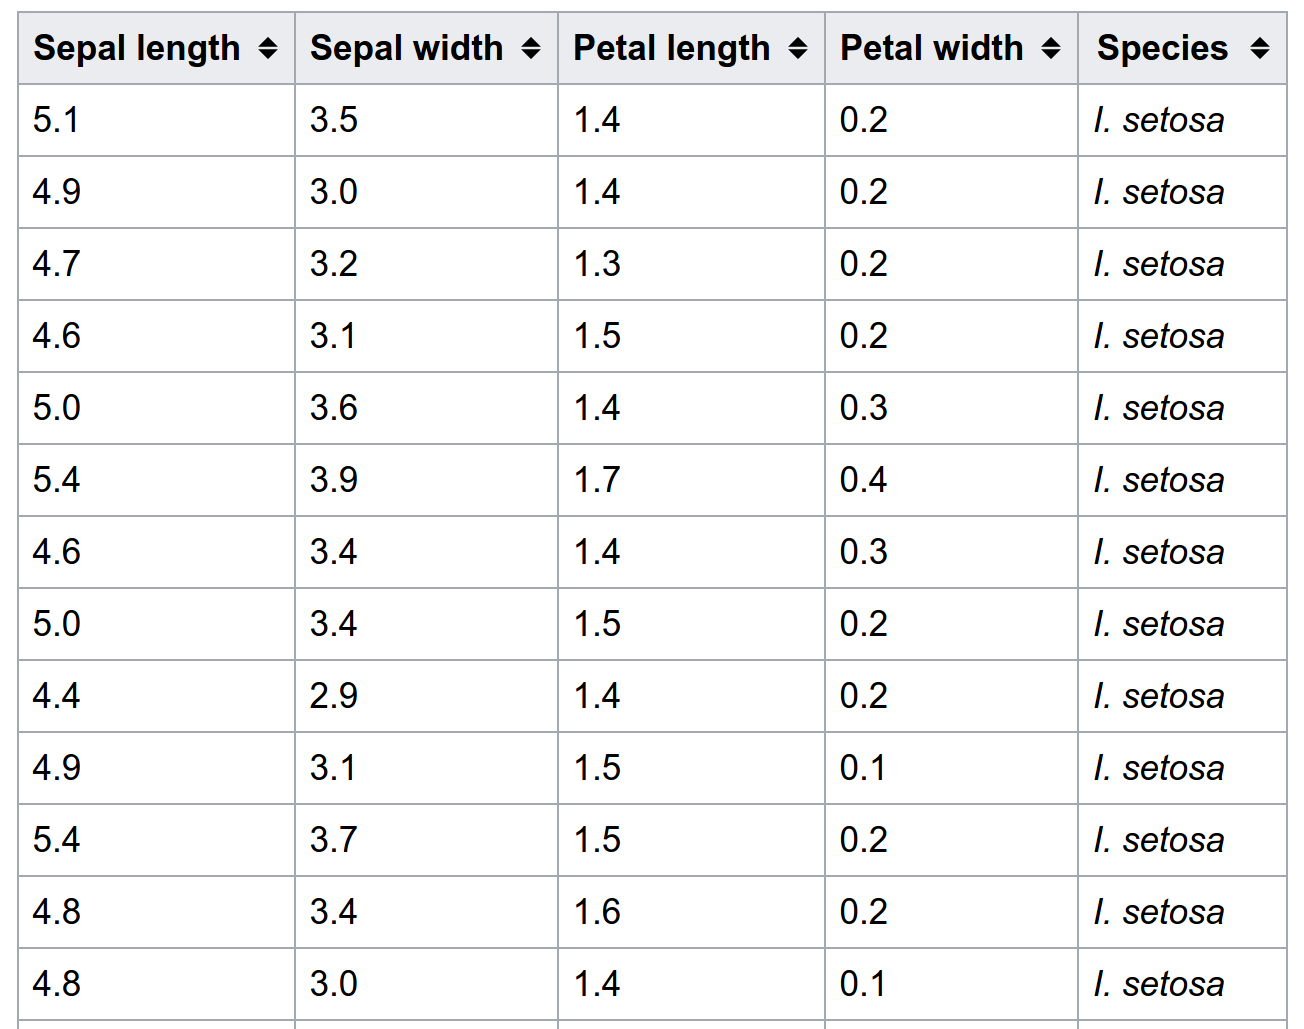
\includegraphics[width=0.75\textwidth]{fisher.png}
  \end{center}
  \caption{The famous Fisher's Iris dataset with first four columns
    being numeric properties of irises and the last column being its
    class. A typical problem then is to predict the class in the last
    column based on the given numeric values in the first four columns}
  \label{fig:iris}
\end{figure}


To illustrate propositional data, let us consider one of the most
classic datasets in statistics and machine learning -- Fisher's Iris
data set\footnote{\url{https://en.wikipedia.org/wiki/Iris_flower_data_set}}.
Figure \ref{fig:iris} depicts a sample of data in the
dataset. Looking carefully at this data, we can establish the
following: every rows is an example and every column is an attribute.
We can also easily see what kind of problem it suggests:
based on the number of values (in the first four columns), a tuple from $R^n$, we need to predict
the class of Iris (in the last column). Many machine learning algorithms
are predictive models. In this thesis we do not work with predictive models.

Classical machine learning algorithms such as the induction of decision trees
\parencite{decision_trees} or Bayesian networks \parencite{pearl} work
with this kind of propositional data and representations.  Propositional representations do not allow to
represent naturally problems involving multiple complex objects
together with the relationships that hold between them. This limitation has been
pointed out by a number of researchers, e.g., in the seminal work of
\textcite{plotkin}, who has introduced  the use of first order logic
for machine learning. Logical and relational learning 
overcomes this limitation by focusing on expressive knowledge
representation languages such as first order logic to handle
relational data \parencite{luc_book}. This approach allows to represent a variable amount of complex objects together with their
relationships -- we refer to this problem setting as \textit{relational}.


Typical machine learning algorithms and data mining systems 
Contrary to this classic machine learning setting with propositional
data, relational learning is looking into a more complex and
interconnected relational data. A real-world example and, probably
very well familiar to the reader, a \textit{spreadsheet} with its formulae is an
excellent example of relational data: it contains a number of
relations or \textit{tables}, and their number is never fixed in
advance, since a spreadsheet might contain an arbitrary number of
them. Also, spreadsheets combine both textual and numeric data. Furthermore,
formulae and constraints over the tables play the role of relationships.

\begin{figure}[thb]
  \begin{center}
    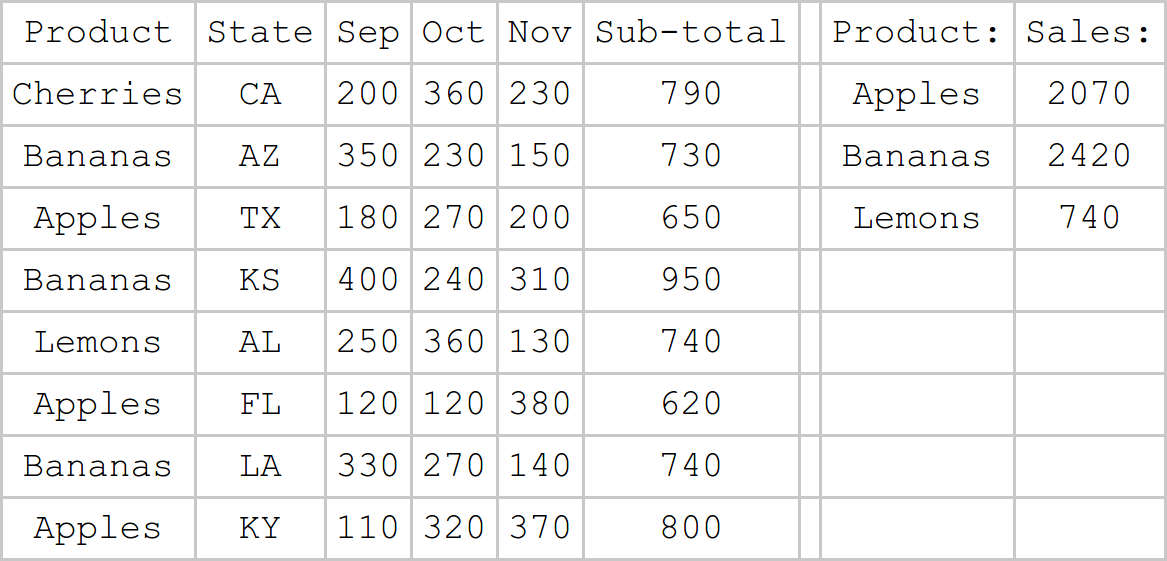
\includegraphics[width=0.75\textwidth]{spreadsheet.png}
  \end{center}
  \caption{A spreadsheet is an example of relational dataset: it has multiple connected tables, constraints between tables, formulae over columns and rows, numeric and non-numeric entries}
  \label{fig:spreadsheet_example_intro}
\end{figure}

Figure \ref{fig:spreadsheet_example_intro} demonstrates this idea:
there are multiple tables connected to each other, the table on the
right has aggregated data over rows in the left table, which means
that generally speaking rows cannot be seen as independent: adding a
row to the first table should update the values in of the right table;
there are various data types present here numeric; categorical and
might have been textual as well. Furthermore, constraints that hold in
a spreadsheet do not have to be functional, i.e., having a form of
$f(\bar x) = y$, where given input $\bar x$ you can always compute
$y$. An example of a non-functional constraint, as we called it here,
is a foreign key. Simply speaking a foreign key constraint enforces
the subset relation. In Figure \ref{fig:spreadsheet_example_intro}, we
see that the right table has an aggregated information over the left
table. Namely there is a \texttt{SUMIF} constraint \footnote{\url{https://support.office.com/en-us/article/sumif-function-169b8c99-c05c-4483-a712-1697a653039b}}, then there is a subset relationship between the column \textit{Product} in the right table and in the left -- it cannot be the case that aggregated information contains a product not listed in the table on the left.
\pubrevend

Depending on the data, one can consider different types of pattern
mining tasks, which we now introduce.

\section{Types of relational mining problems}\label{sec:rel_problems}
In this section we discuss main relational data mining problems that
we investigate in this thesis: relational pattern mining, constraint learning
and relational data factorization.



%   \pubrev
%   A schedule is another example of relational data, which often involves complex constraints.
%   \pubrevend

%   \begin{example}[Examination room scheduling]
%   To make this example concrete, assume that students need to be assigned to
%   auditoria for examinations with professors. Typically, making such a
%   schedule involves dealing with interconnected constraints:
%       \begin{itemize} 
%       \item certain exams
%   must have enough gap time between them 
%       \item rooms can be shared by at most
%       a few courses 
%   \item professors might have their own personal preferences
%   \item university administration might enforce certain administrative and 
%   legal constraints 
%       \end{itemize} 
%       
%   A possible approach is to learn these 
%   constraints by recovering them from
%   a set of positive and negative examples. The number of constraints is
%   not set in advance and the constraint language is typically a rich
%   relational language, for example, a constraint saying that no room is
%   shared by more than three courses at the same time can be expressed in the first
%   order language as
%   \begin{equation*}
%       \forall X,T: \textit{room(X)} \wedge \textit{time(T)} \implies \{ C : \textit{examination}(X,C,T) \wedge \textit{course(C)} \} \leq 3.
%   \end{equation*}
%   \end{example}



\paragraph{Constraint learning} \label{sec:constraint_learning}
Constraint Learning is the research field concerned with finding 
constraints that hold in data
\parencite{constraint_learning,QUACQ,Conacq}. Constraint learning in
relational data is of a great importance to us as we will demonstrate
here.

%Let us outline in simple terms, what constraint learning is about.
%   Similar to the pattern matching problem, we can define 
%   the constraint learning problem as a special case of theory mining:
%   the language of patterns is the set $C$ of possible constraints and

Constraint learning can be formulated in terms of theory mining from
 Section \ref{sec:data_mining} as follows:\\
\begin{definition*}[Constraint Learning]
\begin{mdframed}
 Let $D$ be a dataset, the language of patterns $P$ be the set of
 interesting constraints $C$, 
 $\phi$ be the constraint satisfaction function, 
 then the problem is to find all constraints $c$ in $C$
 such that $\phi(D,c)$ is satisfied, i.e., $c(D)$ holds.
\end{mdframed}
    %\label{def:mining}
\end{definition*}
Simply speaking, constraint learning is pattern mining where patterns
are constraints and the predicate of interest is that the constraints
are satisfied by data.

\sergey{clean up}

%   \begin{example}[Sudoku constraint learning]
%       A well-known Sudoku problem might be hard to model for a person
%       new to constraint programming. A possibility to obtain a model
%       is to it learn from examples. This can be done by providing:
%       \begin{itemize}
%           \item A set of Sudoku solutions
%           \item A set of invalid Sudoku combinations
%           \item An expressive constraint language 
%       \end{itemize}
%   Then, a property of interest is a constraint that holds for all
%       positive Sudoku combinations (all solutions) and for none of
%       the invalid combinations. For example, this can be a constraint of
%       the form
%   \begin{equation*}
%       \forall i: \sum_j x_{ij} = 45
%   \end{equation*}
%       Which shows that the sum of elements in each column is equal to 45
%       (simply the sum of numbers from 1 to 9).
%   \end{example}

%   In case of pattern mining, we enumerate objects on which the property
%   of interest holds: we find graphs or sequences that occur often enough
%   in the data and have certain desired topological properties (for example, being a
%   cyclic graph or have ascending characters). And in constraint learning we find interesting
%   properties that hold in the data (or its parts): given a set of
%   characters, for example, we discovered that the ''ascending
%   constraint`` holds, i.e.,
%   characters are sorted or we found that givens graphs are all cyclic. This shows how two problems are essentially connected.


%   \pubrev
%   \begin{figure}[thb]
%     \begin{center}
%       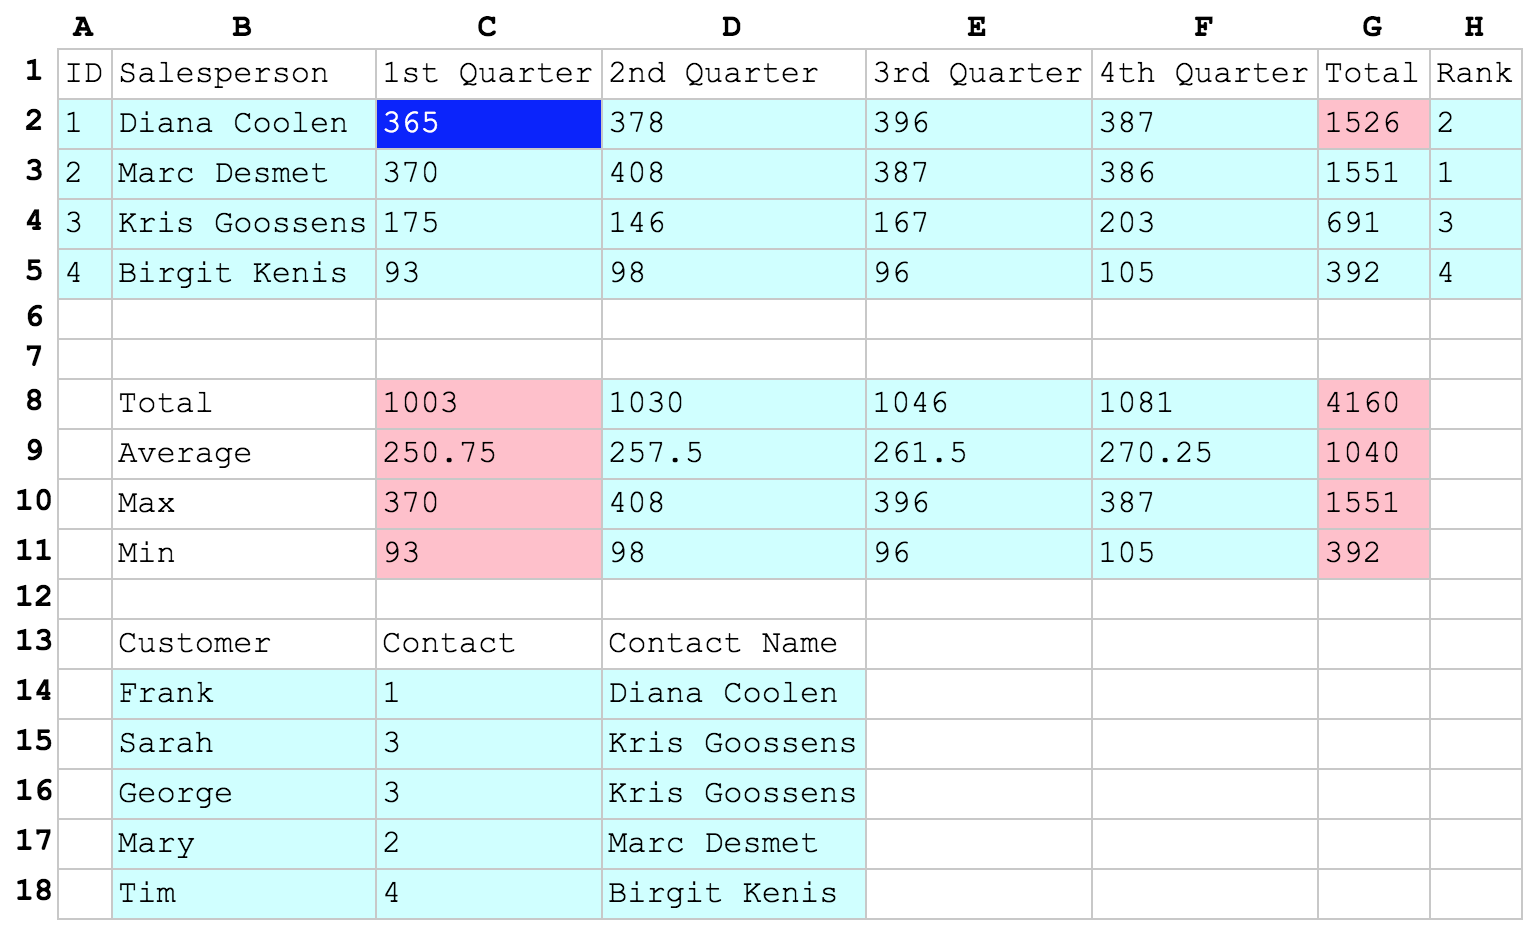
\includegraphics[width=0.75\textwidth]{recomputed.png}
%     \end{center}
%     \caption{A financial report that had certain values originally computed with a software, then if we want to change a cell (in blue), we need to establish all dependencies (i.e., constraints) of this cell and then recompute values that depend upon it (indicated in red), otherwise, data becomes inconsistent with respect to its intended meaning}
%     \label{fig:report_spreadsheet}
%   \end{figure}

Let us illustrate this idea on a spreadsheet in Figure
\ref{fig:spreadsheet_example_intro}. There are two constraints to be
found \texttt{ROWSUM} and \texttt{SUMIF}: the former sums values in rows
in the left table (for columns \textit{Sep}, \textit{Oct} and
\textit{Nov}) and the latter aggregates values (column \textit{Sales}) by category (column
\textit{Product}) in the
right table. Let us indicate why it might be
an important practical problem. Imagine, if we only change one value, the whole data becomes
inconsistent, since there are dependencies in the spreadsheet
to be met, e.g., for example the last column in the left table must be
updated, as well the corresponding category value in the right table. Then, we would like to, first, discover all constraints in the data. Second, update the cell we are interested in and then, third, recompute the values. 

This practical problem is a clear constraint learning problem in a relational setting: we need to enumerate interesting properties, i.e., various spreadsheet constraints, having a form of first order statements and being able to carry out inference on top of a learned model and of relational data (multi-table, interconnected data containing multiple data types). And this is, indeed, the kind of problem that is problematic for classic machine learning and data mining algorithms and require relational methods we develop and investigate here.

For technical details we refer to Chapter \ref{ch:TaCLe} and the work of \textcite{tacle_demo}.
\pubrevend


\paragraph{Relational Pattern Mining}
Let us formulate relational pattern mining problem in terms of theory
mining from Section \ref{sec:data_mining}.\\

\begin{definition*}[Relational Pattern Mining]
\begin{mdframed}
    Let relational data be a relational database $D$, the language of
    patterns $P$ be the set of relational queries $Q$, and 
    $\phi$ be a query satisfaction relation, then the task is to find
    all queries $q$ in $Q$ such that $\phi(q(D))$ evaluates to true.
\end{mdframed}
    %\label{def:mining}
\end{definition*}
A special case of relational pattern mining is 
\textit{frequent pattern mining}. The problem of frequent pattern
mining has as a query satisfaction relation \textit{the minimum frequency
constraint}. Given a frequency threshold $t$ and a predicate of
interest, i.e., what we count, we need to find
all \textit{queries} that occur frequently enough, above the
threshold $t$, in the database $D$. Often we are interested not only in
frequent substructures, but also in substructures that have certain
interesting properties, such as being maximal in size or restricted in
its length or having certain topological properties.

For example, let us assume there is a school database $D$ with three
tables \textit{pupil(PId,FName,LName)},
\textit{class(PId,ClassId,Subject)}, \\
\textit{takes\_test(PId,ClassId,Date,Result)}, which contains
information about pupils, classes they are in and tests they have
taken. Typically, in frequent query mining, we have a target value we
count, in this case, it can be for example PId (Pupil Id), then our
task would be to enumerate the queries that match $D$ often enough.
Let us give a couple of examples how a typical output might look like:

 \begin{figure}[htb]
        
        \begin{tabular}{|c c c|}
            \multicolumn{3}{c}{\textbf{Pupil}}\\
      \hline
            \textbf{PId} & \textbf{Fname} & \textbf{LName}\\ \hline
        p1 &  Nick  & Mason\\
        p2 &  David & Gilmour\\
        p3 &  Syd   & Barret\\
        p4 &  Roger & Waters\\
        p5 &  Richard & Wright \\\hline
    \end{tabular}
     \hfill
        \begin{tabular}{|c c c|}
            \multicolumn{3}{c}{\textbf{Class}}\\
      \hline
            \textbf{PId} & \textbf{ClassId} & \textbf{Subject}\\ \hline
       p1 & c1& drums \\
       p2 & c2& singing \\
       p2 & c3& guitar\\
       p2 & c4& bass \\
       p3 & c2& singing\\
       p3 & c3& guitar\\
       p3 & c5& piano\\
       p4 & c2& singing\\
       p4 & c4& bass\\
       p5 & c2& singing \\\hline
        \end{tabular}
        \hfill
        \begin{tabular}{|c c c|}
            \multicolumn{3}{c}{\textbf{Takes test}}\\
      \hline
            \textbf{PId} & \textbf{ClassId} & \textbf{LName}\\ \hline
        p1 & c1 & 1965\\
        p2 & c2 & 1965\\
        p2 & c3 & 1965\\
        p5 & c3 & 1965\\\hline
    \end{tabular}
    \caption{An example of relational database: music school}
    \label{fig:relational_database_school}
    \end{figure}

\begin{equation*}
\begin{aligned}
q_1(\textit{PId})&\leftarrow \textit{pupil(PId,FName,LName)}.\\
q_2(\textit{PId})&\leftarrow \textit{class(PId,ClassId,Subject)}. \\
q_3(\textit{PId})&\leftarrow \textit{pupil(PId,FName,LName), takes\_test(PId,ClassId,Date,Result)}.\\
q_4(\textit{PId})&\leftarrow \textit{class(PId,ClassId,Subject), takes\_test(PId,ClassId,Date,Result)}.
\end{aligned}
\end{equation*}
The first query $q_1$ is simply taking the table pupil and projecting
on its first column \textit{PId}, $q_2$ does the same for the
\textit{class} table and $q_3$ is making a join between \textit{pupil}
and \textit{takes\_test} on the column \textit{PiD}, $q_4$ is doing the same
but with the tables \textit{class} and \textit{takes\_test}.

Assume our school schema is populated with a data from a music school,
as in Figure \ref{fig:relational_database_school} and we have the
frequency threshold $t=4$, then the queries return corresponding
values:
\begin{equation*}
\begin{aligned}
    q_1(D) = \{ p1, p2, p3, p4, p5 \} \\
    q_2(D) = \{ p1, p2, p3, p4, p5 \} \\
    q_3(D) = \{ p1, p2, p5 \} \\
    q_4(D) = \{ p1, p2, p5 \} 
\end{aligned}
\end{equation*}
Then frequencies of the $q_1$ and of $q_2$ are above the threshold $t=4$
and the frequencies of $q_3$ and $q_4$ are below. That makes $q_1$ and
$q_2$ frequent queries and $q_3,q_4$ are not.

Looking in Figure
\ref{fig:relational_database_school} at the relational data represented
as a relational database, we can contrast this representation of
relational data with a spreadsheet in Figure
\ref{fig:spreadsheet_example_intro}. They are both examples of
relational data but their representations are different. 
Relational databases have a strict schema and structures, while
spreadsheets might have records in columns and rows, it does not
enforce types consistency, constrains and dependencies can be across
multiple tables mixing columns and rows, etc.

\paragraph{Relational Data Factorization}\label{sec:intro_redf}
Another type of problems that is important for this thesis: is that of
matrix and tensor factorizations. Factorizing matrices has a long
history \parencite{matrix_book}, in this thesis we do not focus on
classical continuous decompositions such as SVD or LU, but on its
Boolean version, called \textit{Boolean Matrix
Factorization} \parencite{phd_miettinen}. The main reason for that is
we are going to deal with relational data and non-numeric data in this
thesis. We work with the relational version of BMF under constraints,
we call this problem \textit{Relational Data Factorization}.



In general and not only in the examples presented in this section, the
properties of interconnectedness and expressivity of the constraints
make relational problems hard to model using traditional propositional
approaches, while they can be clearly seen as a first order problem. This gives us confidence that for a number of important problems such as recovering formulae in spreadsheets, factorizing relational data and mining frequent structures in relational data, it is essential to look into richer knowledge representation languages for machine learning.

\section{Declarative approach}\label{sec:declarative_intro}
Many Data Mining problems, and especially pattern mining
problems, are \textbf{combinatorial search problems}, which in turn
have two main components, namely a model and search, which can be
conceptually written as:

\begin{center}
\begin{equation}\label{eq:declarative_schema}
  \text{Combinatorial problem = Model + Search}
\end{equation}
\end{center}

Therefore, it seems natural to model pattern mining problems 
using systems designed to perform search in a declarative manner, such
as \acrlong{cp} \parencite{handbookcp} or \acrlong{asp}
\parencite{whatisasp}. %(which we discuss later in detail).

\pubrev


The declarative approach can be schematically depicted in Eq.
\ref{eq:declarative_schema}, the key idea here is the following: when
we deal with the imperative approach, even a slight change in the
specification of a problem typically leads to a significant change in
the implementation of the algorithm solving this new problem
variation. Contrary to that in the declarative paradigm, we translate
problem specification into a model in an executable declarative language that can
handle various rules and constraints. As a result, a slight change in
the specification translates, ideally, into an additional constraint
being added or a constraint being changed. The key advantage of this
approach is it is easy to solve  closely related problems by varying
the consraints. In our setting, we can think of data
mining problem formulated using mathematical constraints as a
model and \acrlong{cp} (\acrshort{cp}) or \acrlong{asp}
(\acrshort{asp}) engines
as general solvers. In the two following sections we introduce both
formalisms \acrshort{asp} and \acrshort{cp} and their corresponding systems respectively.



\section{Logic programming}\label{sec:logic_programming}
In this section we introduce Logic Programming and \acrlong{asp} that
we have discussed in the context of the declarative approach.


\pubrev
In Eq. \ref{eq:declarative_schema}, we indicate that \textit{a solver}
is going to take care of computing a specification describing the
problem. Also, we already know that \textbf{Data} are relational, i.e., represented as relations. We know that \textit{Logic} naturally can represent relations and relational data in general, then it is logical and natural to use \textit{Logic Programming} as the solving technique in our declarative approach.
\pubrev

In his seminal work Robert \textcite{kowalski} proclaimed:
\begin{center}
  Algorithm = Logic + Control.
\end{center}

%What he meant is quite simple, 
The intuition behind this statement is that
you can turn logical rules into a computational process. 
Why is this important for us? Logic deals with
relations and relational structures, it is naturally designed to
work with relational data. Therefore, if we can combine logic
with computation, we obtain a computational engine that can work in
\pubrev
our relational learning setting: computationally it means that an
executable model we obtain, following the schema in Eq. \ref{eq:declarative_schema}, is close to the original representation of the data and to the specification of the problem.

Ideally, we would like to have such a high level logic programming language that we can write human-like specifications and directly execute them in the system \parencite{denecker}.
\pubrevend

Let us demonstrate how logic programming can be used to model and solve problems. 
\begin{example}[Modelling Sushi preferences with logic]
There are three people: Ronald, Peter and
Alina. We know that people who are not allergic to fish and not vegans like sushi; 
furthermore, we know that Peter is allergic to fish and Ronald is
    vegan. 
Who likes sushi then? We can model this puzzle as a
simple logical implication:

\begin{equation*}
    \begin{aligned}
& \textit{likes\_sushi}(X)~{:}{-}~\textit{person}(X),~\text{not}~
        \textit{allergic}(X), ~\text{not}~\textit{vegan(X)}. \\
&       \textit{allergic(peter)}. \\
&       \textit{vegan(ronald)}.
    \end{aligned}
\end{equation*}

The following notation in Prolog (Programming in logic)
\parencite{birth_of_prolog} mimics the logical implication:

\begin{equation}\label{eq:sushi}
  \forall X: \textit{person}(X) \wedge \text{not }
    \textit{allergic}(X) \wedge \text{not } \textit{vegan}(X)
  \implies \textit{likes\_sushi}(X)
\end{equation}
\end{example}
Therefore, we can think of Logic Programming as an executable Logic, that
we can use to model and solve relational problems.

In this thesis we use modern Logic Programming engines, such
as \acrlong{asp} (\acrshort{asp}) \parencite{ASPbook,whatisasp} and
\acrlong{idp} (\acrshort{idp})
\parencite{idp} %(we explain them in details in the following chapter)
that naturally support constraints and various types of logical
inference.

\pubrev
\acrshort{asp} and \acrshort{idp} are declarative logic programming
formalisms. Contrary to Prolog, which is essentially a full
programming language based on logical inference and provides full
control on the execution flow,  both \acrshort{asp} and \acrshort{idp}
systems fully decouple the problem specification from the execution
flow. In this sense they are closer to \acrlong{cp}. This makes them
an ideal candidate for our general solver in Eq. 
\ref{eq:declarative_schema}, since both of them support relational
data natively and can solve problems declaratively based on a form of
first order logic. We often refer to both paradigms (and to the systems,
associated with them) as \textit{modern logic programming}.

Let us briefly demonstrate the power of \acrshort{asp} on the graph colouring problem (or map coloring problem, as it is known in the popular culture) \parencite{ASPbook}. We assume that \texttt{node/1} encodes nodes of the input graph and \texttt{edge/2} encodes edges of the given graph. First, we declare colours to be used for graph colouring as \texttt{colour(red). colour(green). colour(blue).}, the colors to be used in the \texttt{colouring/2} predicate, then we introduce the following constraint (called a \textit{choice rule}):
\begin{verbatim}
1 {colouring(X,C) : colour(C)} 1 :- node(X).
\end{verbatim}
The rule states that for each node \texttt{X} the predicate \texttt{colouring(X,C)} has one and only one atom to be true for values of \texttt{C} among the colours defined in the predicate \texttt{colour(C)}, simply speaking, this constraint enforces a one-to-one mapping from the nodes (the countries) to the colours.

Then, we need to define a constraint that is saying what mapping is acceptable, in \acrshort{asp}, it is done by defining what is NOT an acceptable solution:
\begin{verbatim}
:- edge(X,Y), colouring(X,C), colouring(Y,C).
\end{verbatim}
If there is an edge between two nodes (countries) \texttt{X} and \texttt{Y} and they are mapped to the same colour \texttt{C}, then it is not a valid solution. As a result, we obtain solutions, where all neighboring nodes of a graph (or neighboring countries) have different colours.
\pubrevend

\section{Constraint programming} \label{sec:cp_intro}
\pubrev
\acrlong{cp} is a declarative methodology for solving combinatorial
problems that also can be used in Eq. \ref{eq:declarative_schema}. The
key difference is that logic programming is typically focused on rules
and inference, while \acrshort{cp} is solely focused on constraint
satisfaction and usually based on a pre-defined set of constraint
primitives (such as comparison, sets operations, etc). In this thesis
we prefer constraint programming over logic programming for
numeric-heavy problems and in all other cases we use logic programming \acrshort{asp} or \acrshort{idp}.
\pubrevend

The essence of the \acrshort{cp} methodology consists of writing a set of
constraints, such as $X + Y > Z$, and inferring a solution to them, such
as $X = 1, Y = 2$ and $Z = 0$. This set of constraints is referred as
a \textit{specification} or a \textit{model}; for this, multiple \acrlong{cp}
languages exist, such as MiniZinc \parencite{minizinc} or Essence
\parencite{essence}. A \textit{solution} for
a model is an assignment, as for example, the one we just indicated, that satisfies
\textit{all} constraints. This general methodology is declarative,
since a user writes a set of constraints corresponding to the
properties of her problem and a \acrshort{cp} solver is looking for a
solution: this clearly demonstrates that it is the task of the solver
to figure out \textit{how} to find a solution, while it is the user's
responsibility to specify \textit{what} the problem is in terms of
writing these constraints.

\begin{example}[MiniZinc CP program]
    Let us illustrate how constraint programming can solve problems on
    a small example of the subset sum problem using the MiniZinc
    system.\footnote{\url{https://github.com/MiniZinc}, see Examples} 

The problem is the following: given a list of numbers and a target
    value, we need to find a subset of these numbers that sum up to
    the target value.
    \begin{minipage}{\linewidth}
    \begin{lstlisting}[caption=An example of a MiniZinc program, label=lst:example_asp_program,basicstyle=\ttfamily]
array[int] of int: number;
int: target;

set of int: NUMBER = index_set(number);
var set of NUMBER: selected;

constraint sum(i in selected)
              (number[i]) = target;
solve satisfy;

output [show(selected)];
\end{lstlisting}
\end{minipage}
The most important part of program in the \texttt{constraint}
part, where we state that the sum of selected numbers is equal to
the target value. The rest is variable declaration and the index
set computation -- technical details at this point.
\end{example}


\pubrev
\section{Common traits}\label{sec:common}
There is a number of common traits and assumptions that the problems, we
investigate in the thesis, share. Typical machine learning algorithm
make use of the, so called, single-tuple single-table assumption. This
assumption states that the data can be represented using
attribute-value pairs. As we have demonstrated the problems we
consider break this assumption. This indicates, the first, common
feature -- they are all relational data  mining problems. 

Second, the pattern minng problems we investigate are a form of combinatorial search and
enumeration problems: we are looking for certain interesting patterns that hold in the data under constraints, e.g., all maximal
(in size) conjunctive queries that hold in the data frequently enough
or in case of tabular constraint learning we enumerate all spreadsheet
formulae (which can be viewed as constraints, see Theory Mining in
Section \ref{sec:data_mining}) that hold between
spreadsheet tables.


Third, all of these problems, we investigate, are relational problems under a
broad variety of constraints, e.g., discovering constraints in tabular
data is not limited to only the list of specified constraints but it
is designed to support the whole \textit{language} of tabular
constraints, i.e., new constraints can be added there in a declarative
manner in the accordance with the \textit{elaboration tolerance}
principle by \textcite{elaboration_tolerance}. In the same way
relational pattern mining is not limited only to its core version of
finding frequent patterns (such as graphs, queries, sequences or
itemsets) but also in finding its \textit{condensed} (such as maximal,
closed, free, etc) representations
under various constraints (such as length, size, or topological
constraints)

Fourth, as we have just indicated, our solutions are declarative in
nature, as indicated in Eq. \ref{eq:declarative_schema} Once we modify
the problem by adding an extra constraint or feature, we do not have
to modify the algorithm completely (as so often happens in the imperative approach \parencite{gspan,clospan}).

Last but not least is the way we approach them, our approach is based
on declarative constraint and logic programming. We demonstrate how
our pattern mining problems can be modelled using modern
logic and constraint programming systems such as \acrshort{asp} and \acrshort{idp}. In addition to the mathematical models
of the relational problems, we provide an evaluation of the
 performance of the resulting systems using an extensive experimental evidence on the behaviour of such systems. To the best of our knowledge, this is the first empirical study of such scale investigation applications of modern logic programming to relational data mining problems.
\pubrevend

\section{Contributions}\label{sec:contributions}
Given the abundance of relational data (such as spreadsheets, graphs,
databases and logical structures) for various machine learning and data
mining problems, and the success in the development of declarative solvers (such
as \acrshort{asp}, \acrshort{idp} and \acrshort{cp}) a
natural question arises: \textit{``How can we declaratively model and
solve relational data mining problems using declarative programming
techniques?''}. 

The \textbf{main contribution} of this thesis is in the application of
modern logic programming languages, such as \acrshort{asp} and
\acrshort{idp}, to these novel relational data mining problems.


Concretely, we investigate how the following data mining problems
can be modelled and solved using a declarative approach based on
logic programming.
\pubrev
\begin{itemize}
    \item \cone: What are the challenges and advantages of generalizing
    classic data mining problems, such as the Boolean Matrix
    Factorization problem, into the relation setting? We address this
        question by proposing \textbf{Relational Data Factorization.}
  \item \ctwo: How can the constraint learning problem be formulated
   and modelled in the relational setting, where data is
   represented as spreadsheets, i.e., connected relations, and constraints are
   tabular Excel-like formulae? We propose as an answer \textbf{Tabular Constraint Learning.} 
  \item \cthree: Can we model and automatically complete a partially specified logic program?
      A partially specified program is a program where certain
        parts are marked as uncertain. We propose a declarative approach to
        this problem, called \textbf{Sketched Answer Set Programming}.
   \item \cfour:
%  Similarly to unstructured constraint-based itemset mining: 
    How can we apply declarative relational mining
    techniques, such as logic programming, to structured frequent pattern mining, such as sequence, graph
    and query mining? We introduce an \textbf{ASP-based Relational
        Pattern Mining Model} as a possible solution to this problem.
\end{itemize}
\pubrevend

Addressing \cone, \textbf{Chapter} \ref{ch:ReDF} presents the novel problem of Relational Data
Factorization. It demonstrates how this problem generalizes various
data mining problems such as Database Tiling and Boolean Matrix
Factorization. We start with the most basic setting and demonstrate
how various problems can be modelled within the framework by adding
or modifying the constraints. Then, we show how the framework can be
used for new and interesting applications and propose Answer Set
Programming as a method to solve the problem in the general case.
For each problem we provide extensive experimental evidence,
including solver parameter tuning. The chapter consists of the
research previously published in the following paper:

\begin{addmargin}[2em]{2em}

Sergey Paramonov,  Matthijs van Leeuwen, Luc De Raedt: Relational data
factorization, Machine Learning, Springer, December 2017, Volume 106,
    Issue 12, pp 1867–1904.

\end{addmargin}



With regards to \ctwo,  \textbf{Chapter} \ref{ch:TaCLe} introduces  the novel problem of
Tabular Constraint Learning and the system, called TaCLe (pronounced
as the word ``tackle''). The problem setting is straightforward to
explain: we have an Excel file with formulae. The file is imported as
CSV. The formulae are lost. Can we reconstruct them? We can already 
see that the problem setting is different from the standard machine
learning problem. In a spreadsheet, columns are no longer variables
and rows are no longer records. Textual and numeric data are mixed.
Spreadsheet functions, such as Fuzzy-lookup, are unorthodox and unseen in
the constraint programming and constraint learning research communities.

The chapter consists of the research previously published in the following papers:

\begin{addmargin}[2em]{2em}
Samuel Kolb (*), Sergey Paramonov (*), Tias Guns, Luc De Raedt:
  Learning constraints in spreadsheets and tabular data. Machine
  Learning 106 (9-10), pages 1441-1468, 2017.


Sergey Paramonov (*), Samuel Kolb (*), Tias Guns, Luc De Raedt:
TaCLe: Learning constraints in tabular data. 
 Proceedings of the 2017 ACM on Conference on Information and
    Knowledge Management, CIKM 2017, pages 2511-2514, Sheridan
    Communications, Conference on Information and Knowledge Management
    (CIKM), Singapore, 6-10 Nov 2017.

\pubrev
(*) -- equal contribution.
\pubrevend
\end{addmargin}




%   we look into a more practical setting.
%   Typically, machine learning and data mining algorithms' assumptions make the i.i.d.
%   (independent identically distributed) assumption, which of course
%   breaks in the relational setting. If we look at a spreadsheet, it 
%   typically consists one or more tables with relationships between them or
%   within the table itself, usually
%   in a form of a formula, a macro or of some other constraint (e.g., a
%   C\# or VB script). If we
%   want to detect these connections between tables or their parts, we
%   have to make the model able to work with spreadsheet data, 
%   formulae and tabular constraints. This setting, referred to as the
%   \textit{Tabular constraint learning}, breaks the standard
%   machine learning and data mining algorithms and 
%   makes the problem essentially relational.

Addressing \cthree:  \textbf{Chapter} \ref{ch:sketching} introduces the novel problem of
Sketched Answer Set Programming. The idea of sketching takes root in
imperative programming, when a function in C or Java has a part of it,
typically a constant, left unspecified. A user then provides a number
of examples for this sketched constant to be filled in with a
correct value satisfying the examples. Inspired by this approach, we
introduce Sketched Answer Set Programming, where a user writes a
regular program but with certain parts such as constants, predicates
or operators are left uncertain. Then, we rewrite this sketched
program into a regular \acrlong{asp} program, i.e., we use a standard ASP solver
to complete sketches.


The chapter consists of the research previously published in the following papers:
\pubrev
\begin{addmargin}[2em]{2em}
  Sergey Paramonov, Christian Bessiere, Anton Dries, Luc De Raedt:
  Sketched Answer Set Programming. 30th International Conference on Tools with Artificial Intelligence, IEEE, 2018, International Conference On Tools With Artificial Intelligence, Volos, Greece 
\end{addmargin}
\pubrevend



%   assume we already have a logic programming or a
%   constraint model of a relational
%   data mining problem due to relational dependencies in the data which 
%   force to give up the i.i.d. assumption and, as a consequence,
%   standard techniques. When something changes over time or due to changes in the specification, we would like
%   to be able to indicate uncertainty in some parts of the model and use
%   the system itself. These
%   uncertain or, \textit{open}, parts are called \textit{sketched} and
%   the whole sketched model is referred to as a \textit{sketch} and the related
%   problem as \textit{constraint sketching}. We propose the problem of and
%   a learning technique for \acrlong{skasp}.


Finally, with respect to \cfour, \textbf{Chapter} \ref{ch:StructuredMining} introduces a logic
based approach to structured pattern mining. The idea to apply general
solvers to pattern mining takes root in the work of
\textcite{declrativeapproach}, where Constraint Programming is applied to
Itemset Mining. Contrary to itemset mining, where objects do not have
any particular structures, structured mining studies mining patterns
in sequences, trees, graphs, etc. First, we introduce a general
mathematical model of general frequent pattern mining based on the logical formulation of
the constraints. Second, we show that the model can be hybridized by
using our generic framework together with specialized solvers
developed for particular pattern mining problems.

The chapter consists of the research previously published in the following papers:
\begin{addmargin}[2em]{2em}
\pubrev
Sergey Paramonov, Daria Stepanova, Pauli Miettinen: Hybrid ASP-based
    Approach to Pattern Mining. Theory and Practice of Logic
    Programming, 2018.
\pubrevend

Sergey Paramonov, Matthijs van Leeuwen, Marc Denecker, Luc De Raedt:
An Exercise in Declarative Modelling for Relational Query Mining.
Lecture Notes in Computer Science, volume 9575, pages 166-182,
    Springer, Inductive Logic Programming, Kyoto, 20-22 August 2015.

Sergey Paramonov, Daria Stepanova, Pauli Miettinen:
Hybrid ASP-Based Approach to Pattern Mining.  
Rules and Reasoning - International Joint Conference, RuleML+RR 2017,
    Springer Lecture Notes in Computer Science (LNCS), pages 199-214,
    Springer, 2017, RuleML+RR 2017: International Joint Conference on
    Rules and Reasoning, July 12-15, London, UK.

Tias Guns, Sergey Paramonov, Benjamin Negrevergne: On declarative
    modelling of structured pattern mining, AAAI Workshop on
    Declarative Learning Based Programming, Phoenix, Arizona USA, 13
    February 2016.

Sergey Paramonov, Chen Tao, Tias Guns: Generic mining of condensed
    pattern representations under constraints, Young Scientist's
    Second International Workshop on Trends in Information Processing
    (YSIP2), pages 168-177, CEUR Workshop Proceedings, Young
    Scientist's International Workshop on Trends in Information
    Processing, Dombai, Russia, 16-20 May 2017.

Matthias van der Hallen, Sergey Paramonov, Michael Leuschel, Gerda
    Janssens: Knowledge representation analysis of graph mining,
    Bogaerts, Bart; Harrison, Amelia (eds.), Proceedings of ASPOCP
    2016, pages 55-76, Workshop on Answer Set Programming and Other
    Computing Paradigms, New York, 16 October 2016.
\end{addmargin}




%   if we look at the area of itemset mining, where \acrlong{cp}
%   has been successfully applied, then the natural question to ask is:
%   if \acrshort{cp} has been successful for unstructured, or
%   non-relational, pattern mining, can we model its \textit{structured},
%   or \textit{relational} version, using logic programming? To answer
%   this question we look into \textit{sequence}, \textit{graph} and
%   \textit{query mining} and attack them using logic programming and
%   hybrid approaches based on logic programming.

%   \paragraph{Structure of the thesis}
%   \textbf{Chapter} \ref{ch:background} introduces background information
%   on Logic, Answer Set and Programming and Pattern Mining.

\textbf{Chapter} \ref{ch:conclusions} summarizes the thesis and
discusses future work possibilities.

\section{Datasets, code and experimental results}\label{sec:datasets}
In order to make results repeatable and to follow the Open Source
spirit, we have opened and published the datasets, use-cases,
meta-data and other useful information.
They can be found in the following GitHub repositories:
\pubrev
\begin{itemize}
\item \url{https://github.com/SergeyParamonov/TaCLe} with materials for Chapter ''Learning Constraints in Tabular Data''
\item \url{https://github.com/SergeyParamonov/sketching} with materials for Chapter ``Sketched Answer Set Programming''
\item \url{https://github.com/SergeyParamonov/StructuredMiningASP}
    with materials for Chapter ``Relational Pattern Mining''
\item \url{https://github.com/SergeyParamonov/RelationalDataFactorization} with materials for Chapter ``Relational Data Factorization''
\end{itemize}
\pubrevend
\cleardoublepage
% vim: tw=70 nocindent expandtab foldmethod=marker foldmarker={{{}{,}{}}}
